\subsubsection{API Gateway}

L'API Gateway è il cuore della piattaforma. Il suo compito è, previa verifica dei privilegi e aggiornamento del database SLA, reindirizzare le chiamate dell'utilizzatore finale e instradarle verso il fornitore del microservizio.  La necessità del passaggio per un gateway centralizzato è per motivi di data analysis nonchè di controllo della validità delle chiavi. \\

L'API Gateway è un package del back-end, tuttavia l'approccio a microservizi adottato ci consente di descriverlo come un entità a sè stante. Esso è composto dai campi dati per mantenere in coda le chiamate e un servizio interno che si occupa di effettuare le operazioni di verifica chiave, verifica e scrittura SLA, forwarding delle chiamate e forwarding delle risposte.  \\

Il package principale per il servizio API Gateway è rappresentato dal seguente diagramma UML:


\begin{figure}[!htbp]
	\centering
	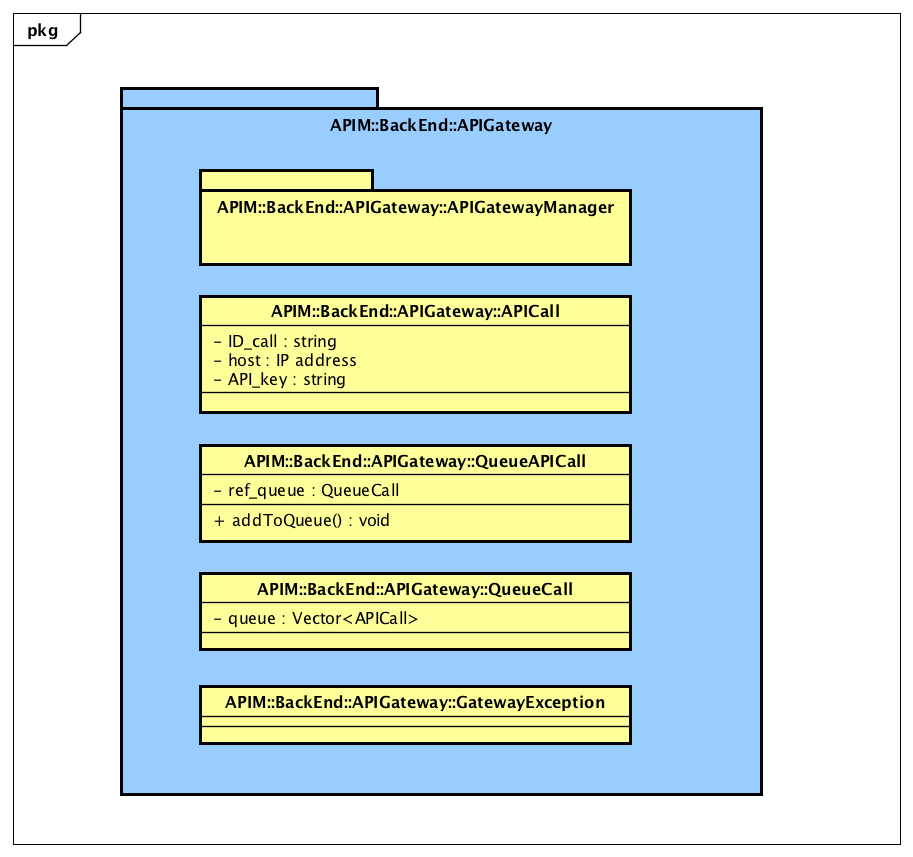
\includegraphics[scale=0.45]{UML/DiagrammiPackage/ApiGateway.png}
	\caption{ApiGateway}
\end{figure}


Il package APIGateway, che rappresenta il servizio omonimo, contiene il seguente package:

\begin{itemize}
	\item \textbf{ApiGatewayManager}: questo package si occupa gestire le richieste in arrivo, instradare la richiesta al microservizio richiesto e di ovviare in modo opportuno alle condizioni di errore.
\end{itemize}

\paragraph{APICall}
\begin{itemize}
	\item \textbf{Funzione del componente}: la classe si occuper\`{a} di istanziare un oggetto che rappresenta la chiamata a un microservizio ricevuta da un client;
	\item \textbf{Attivit\`{a} svolte e dati trattati}: la classe contiene un id che identifica univocamente una chiamata, un indirizzo IP per sapere dove restituire la risposta della chiamata e la API Key dell'utente;
	\item \textbf{Relazioni d'uso di altri componenti}: \textit{QueueCall}, \textit{QueueAPICall}.
\end{itemize}

\paragraph{QueueAPICall}
\begin{itemize}
	\item \textbf{Funzione del componente}: la classe si occuper\`{a} di istanziare una oggetto che contiene un riferimento a un oggetto QueueCall, il cui numero di istanze \`{e} finito;
	\item \textbf{Attivit\`{a} svolte e dati trattati}:  Il suo compito principale sar\`{a} aggiungere la richiesta a un microservizio in coda tramite un riferimento a \textit{QueueCall};
	\item \textbf{Relazioni d'uso di altri componenti}: \textit{QueueCall}.
\end{itemize}

\paragraph{QueueCall}
\begin{itemize}
	\item \textbf{Funzione del componente}: questa classe istanzier\`{a} un numero finito di oggetti, di numero controllato, in modo da garantire un buon servizio, che conterr\`{a} una struttura dati Vector, usata per contenere le APICall;
	\item \textbf{Attivit\`{a} svolte e dati trattati}:  Il suo compito principale sar\`{a} registrare la richiesta a un microservizio;
	\item \textbf{Relazioni d'uso di altri componenti}: \textit{APICall}.
\end{itemize}

\paragraph{GatewayException}
\begin{itemize}
	\item \textbf{Funzione del componente}: questa classe istanzier\`{a} un oggetto che rappresenta una condizione d'errore nella richiesta ricevuta;
	\item \textbf{Relazioni d'uso di altri componenti}: \textit{APICall}.
\end{itemize}

\paragraph{GatewayManager}
\begin{figure}[!htbp]
	\centering
	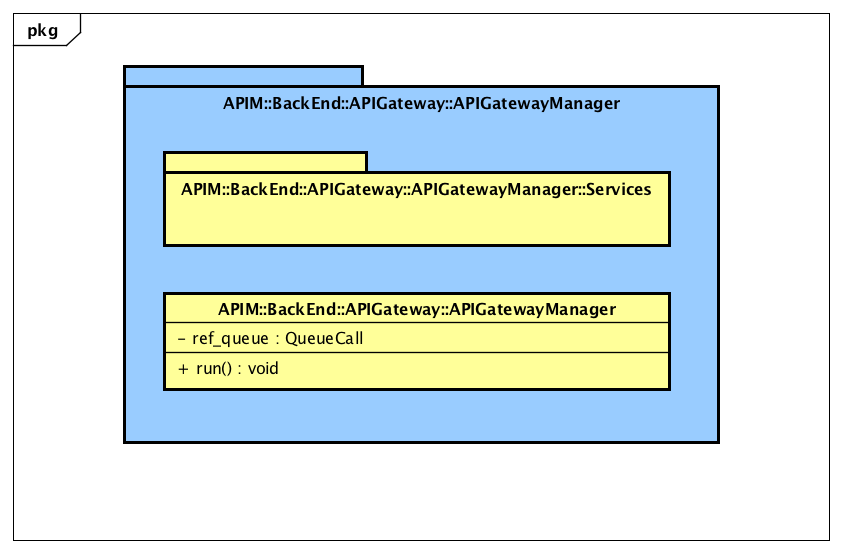
\includegraphics[scale=0.45]{UML/DiagrammiPackage/APIGatewayManager.png}
	\caption{ApiGateway}
\end{figure}

Il package APIGatewayManger, che rappresenta il servizio omonimo, contiene il seguente package:
\begin{itemize}
	\item \textbf{ApiGatewayManager}: questo package si occupa gestire le richieste in arrivo, instradare la richiesta al microservizio richiesto e di ovviare in modo opportuno alle condizioni di errore. Il suo compito \`{e} anche quello di monitorare  l'utilizzo dei microservizi.
\end{itemize}

\subparagraph{ApiGatewayManager}
\begin{itemize}
	\item \textbf{Funzione del componente}: questa classe istanzier\`{a} un oggetto che rappresenta un task ed avr\`{a} la funzione di avviare un Thread che gestir\`{a} le richieste correnti all'APIGateway usando i services;
	\item \textbf{Relazioni d'uso di altri componenti}: \textit{QueueCall}.
\end{itemize}

\subparagraph{Services}
\begin{figure}[!htbp]
	\centering
	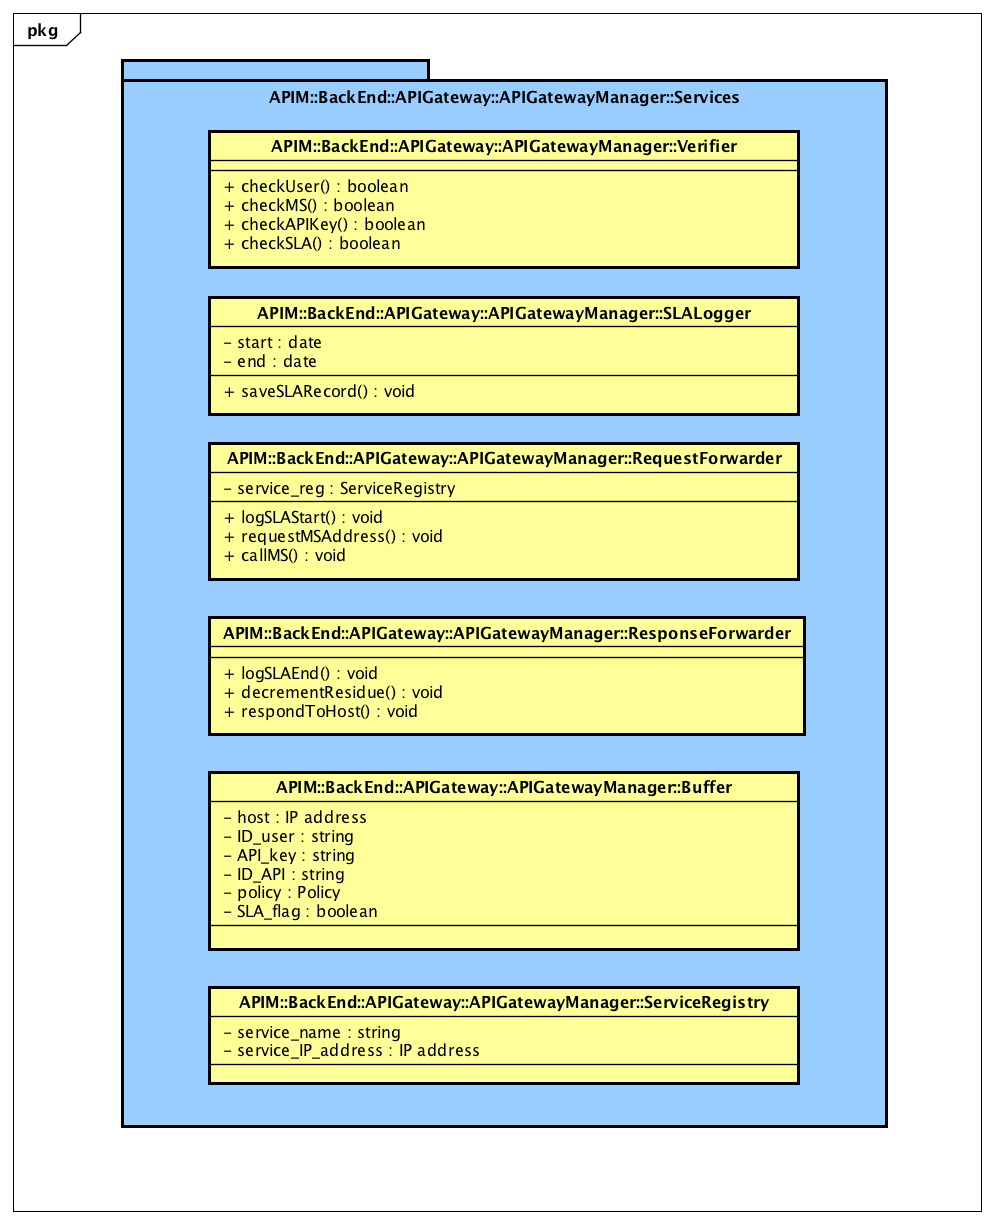
\includegraphics[scale=0.45]{UML/DiagrammiPackage/ApiGatewayManagerServices.png}
	\caption{ApiGateway}
\end{figure}
\FloatBarrier

\subparagraph{Verifier}
\begin{itemize}
	\item \textbf{Funzione del componente}: la classe rappresenta un microservizio che si occupa di verificare che la richiesta ricevuta all'ApiGateway sia valida;
	\item \textbf{Attivit\`{a} svolte e dati trattati}: la classe controller\`{a} che l'utente sia un utente valido, che il microservizio esista e sia attivo, che l'ApiKey dell'utente non sia scaduta e la SLA associata alla richiesta sia rispettata;
	\item \textbf{Relazioni d'uso di altri componenti}: RequestForwarder.

\end{itemize}

\chapter{SLALogger}
\begin{itemize}
	\item \textbf{Funzione del componente}: la classe si occuper\`{a} di istanziare un oggetto che rappresenta gli intervalli di inizio e fine di una chiamata a un microservizio;
	\item \textbf{Attivit\`{a} svolte e dati trattati}:  la classe avr\`{a} il compito di salvare in un buffer la data di inizio e fine di una chiamata sulla base dell'id di quella chiamata, dati che ricever\`{a} dagli altri componenti dell'APIGateway;
	\item \textbf{Relazioni d'uso di altri componenti}: \textit{RequestForwarder}, \textit{ResponseForwarder}.
\end{itemize}

\chapter{RequestForwarder}
\begin{itemize}
	\item \textbf{Funzione del componente}: la classe si occuper\`{a} di istanziare un oggetto che avr\`{a} il compito di instradare la richiesta ricevuta al microservizio corretto e salvare i dati della richiesta;
	\item \textbf{Attivit\`{a} svolte e dati trattati}: la classe, sulla base delle informazioni dell'IP recuperato dal ServiceRegistry, inoltrer\`{a} la richiesta ricevuta al microservizio corretto e richieder\`{a} allo SLALogger di salvare i dati relativi al tempo di inizio della richiesta;
	\item \textbf{Relazioni d'uso di altri componenti}: \textit{ServiceRegistry}, \textit{SLALogger}.
\end{itemize}

\chapter{ResponseForwarder}
\begin{itemize}
	\item \textbf{Funzione del componente}: la classe si occuper\`{a} di istanziare un oggetto che avr\`{a} il compito di ricevere la risposta da parte di un microservizio sulla base di una chiamata al microservizio e salvare i dati relativi alla richiesta;
	\item \textbf{Attivit\`{a} svolte e dati trattati}: comunica con lo SLALogger per salvare i dati circa il tempo di fine della richiesta, o in caso di esito negativo della richiesta di apporre il corretto flag per segnalarlo. Inoltra poi i dati di risposta al client richiedente;
	\item \textbf{Relazioni d'uso di altri componenti}: \textit{SLALogger}.
\end{itemize}

\chapter{Buffer}
\begin{itemize}
	\item \textbf{Funzione del componente}: la classe si occuper\`{a} di istanziare una oggetto che rappresenta un buffer 
	\item \textbf{Attivit\`{a} svolte e dati trattati}: contiene l'IP dell'host, l'ID dell'utente che ha effettuato la richiesta, la API Key e il suo id, la policy di vendita e un flag relativo alla SLA per indicare se rispettata o meno;
	\item \textbf{Relazioni d'uso di altri componenti}.
\end{itemize}

\chapter{ServiceRegistry}
\begin{itemize}
	\item \textbf{Funzione del componente}: la classe si occuper\`{a} di istanziare una classe oggetto che rappresenta un microservizio;
	\item \textbf{Attivit\`{a} svolte e dati trattati}: la classe fornisce le generalit\`{a} del microservizio: il suo IP e nome;
	\item \textbf{Relazioni d'uso di altri componenti}: \textit{RequestForwarder}.
\end{itemize}





